\documentclass[11pt]{article}
\setlength{\parskip}{1em}
\usepackage{amsmath}
\usepackage{gensymb}
\usepackage{amsthm}
\usepackage[left=1in, right=1in, top=1in]{geometry}
\usepackage{graphicx}
\usepackage{wrapfig}
\usepackage{lipsum}
\usepackage{listings}
\usepackage{titling}
\usepackage{datetime}
\usepackage{float}
\usepackage{amssymb}
\usepackage[export]{adjustbox}
\usepackage{caption}
\usepackage{subcaption}
\usepackage{pdfpages}

\usepackage{url}
\usepackage{fancyhdr}
\usepackage[font={small,it}]{caption}
\captionsetup{justification   = raggedright,
	singlelinecheck = false}

\graphicspath{ {D:\Digitial_Image_Processing\Final_Paper} }


\theoremstyle{definition}
\newtheorem{defn}{Definition}[section]

\definecolor{dkgreen}{rgb}{0,0.6,0}
\definecolor{gray}{rgb}{0.5,0.5,0.5}
\definecolor{mauve}{rgb}{0.58,0,0.82}




\begin{document}
	\lstset{language=python} 
	\title{LiDAR: Analysis and Classification}
	
	\author{Steven Spiegel}
	\date{\today}
	\maketitle

	\begin{abstract}
		LiDAR (Light Detection and Ranging) is ubiquitous in its use and applications.  Some of its applications is in computer vision and robotics, surveying, emergency management, and object classification.  this project aims to introduce the reader into the science of LiDAR, processing tools, and applications.  In particular, this paper will look at PDAL (Point Data Abstraction Library) and its use in point cloud processing and application.  The point cloud in question can be found and downloaded on the PDAL website. In conjunction with Python and Jupyter Notebook, this paper seeks to efficiently remove outliers, segment the ground, and classify the remaining points of an airborne LiDAR collection into 2 different classes: Buildings and vegetation. The full algorithm can be found in the "Lab.ipynb" jupyter notebook.  
	\end{abstract}
	\newpage
	\section{Introduction}\label{sec:intro}
	LiDAR (Light Detection and Ranging) is used in numerous scientific contexts, particularly in the realm of computer vision and surveying.  At it's heart, LiDAR measures the distances between transmitted and received signals.  There are several main types of LiDAR:
	\begin{enumerate}  
		\item Pulse: Emits a pulse and measures the time between hitting a target and the return time. 
		\item Phase: Measures distances using interferometry. 
		\item Geiger: Use sensors that are triggered by photons. 

	\end{enumerate}
	The mode of LiDAR used in this project is pulse based \cite{pdal}. 
	\\\\
	In addition to the different types of LiDAR, there are a number of different collection techniques.  The four primary types are terrestrial, airborne, mobile, and Unmanned Aerial Systems (UAS).  Terrestrial collects require the use of reflectors or planar regions to register scans together. The main struggle with this type of collect is the amount of work in moving the scanner from different scan positions.  However, these scanners often have ranges that are on the kilometer scale, allowing for massive data collects.  Mobile scans use the power of Robotic Operating Systems and feature matching to create a point cloud.  As the price of small LiDAR scanners and Unmanned Aerial Systems have become increasingly affordable, UAS LiDAR collection is becoming more common.  What would usually take days for surveyors to collect with a terrestrial scanner, UAS can collect in hours.  A plethora of software suites exist to process the LiDAR data for relative accuracy as well as absolute accuracy.    
	\\\\
	In this context, we are focused on classifying point clouds once they have been collected and processed.  There are a number of techniques to accomplish this.  In general, the strategy is as follows: Classify the ground, segment the point cloud, and classify the segments, as demonstrated in the master's thesis of Nina Varney \cite{varney}.  Other strategies can be taken to classify point clouds, such as PointNet, which utilizes an Convolution Neural Network to segment and classify point clouds \cite{PointNet}.  In our case, we directly classify the ground and then use the geometric properties of the remaining points to identify what class they should be in.  This is a more simplistic method than shown in \cite{PointNet} and \cite{varney}, however it will be sufficient for our purposes.  We know that in our scene we are only interested in classifying the vegetation and buildings.  Hence, we can mainly focus on looking at the geometric properties of the points themselves and then deduce what class they should be in.  The general strategy for processing the point cloud is as follows:  
	\begin{enumerate}  
	\item Remove outliers via a statistical or distance method.
	\item Use morphological filtering and return numbers to classify ground returns.
	\item Use point covariance to determine normal planes of remaining points.
	\item Use Singular Value Decomposition of the Covariance Matrix to determine dimension of the points.
	\item Classify based on the dimension of points.
\end{enumerate}
In order to accomplish this, we will employ PDAL pipelines which are written as JSON files and used in a Jupyter Notebook  \cite{pdal}.  PDAL has a python interface that allows one to create custom python code in addition to PDAL pipelines.  These functions are written in C++, but PDAL allows python to be used in addition to the pipelines.
\\\\
The Methods section will demonstrate these methods as well as give a brief discussion on the theory of each one.  Then, a basic PDAL pipeline will be demonstrated.  For the purpose of this exercise, our goal is to classify outliers, ground, buildings, and vegetation. 
\section{Dataset Description}\label{sec:dataset}
We will be classifying an airborne LiDAR collect called \texttt{CSite1\char`_orig-utm} \cite{pdal}. This can be found on the PDAL website and is an often used LiDAR data collection set. The projection is UTM zone 32N with an average point spacing of $~0.75\text{ }m$, area of $~781062\text{ }m^2$, and an average of $~1.72\text{ }\frac{pt}{m^2}$.

\section{Methodology}\label{methods}
The theoretical approach to point cloud classification is enumerated in section \ref{sec:intro}.  We will use a PDAL pipeline in addition to python processing in Jupyter Notebook to remove outliers, classify ground returns, and classify vegetation and buildings.  The next part of the methods section will give theoretical primers to each one of these tasks.  Example PDAL pipelines are detailed as well.  
\subsection{Outliers}\label{sub:outliers}
The first thing we need to do is to classify the outliers.  Outliers are noise points that aren't attributed to things we are interested in.  In airborne LiDAR this could be due to dust, birds, etc.  Hence, the first step is to eliminate outliers.  There are 2 primary methods used in PDAL: Statistical and Radial \cite{pdal}.
\subsubsection{Statstical}\label{subsub:stat}
Statistical Outlier Removal requires 2 calculations across the point cloud.  On the first pass, for point cloud $P$ with $n$ points, and for each point $p_i$ for $i\in 1 \ldots N$, the mean distance $\mu_i$ is computed for $k$ nearest neighbors.  Then, we calculate the global mean of means in the following:
\begin{equation}\label{eqn:average} 
\mu=\dfrac{\sum_{i=1}^{N} \mu_{i}}{N} 
\end{equation}
and the standard deviation ($\sigma$) is defined as
\begin{equation}\label{eqn:std} 
\sigma=\sqrt{\dfrac{\sum_{i=1}^{N} (\mu-\mu_{i})^2}{N-1}} 
\end{equation}

Thus, the threshold ($t$) for outlier classification is as follows:
\begin{equation}\label{eqn:threshold}
t=\mu+\sigma m
\end{equation}
where $m$ is a user defined input.  Thus, we have the following criteria for a statistical outlier:
\begin{equation}\label{eqn:stat_rule}
outlier_{i}=\begin{cases}
true & \text{if $\mu_{i}>t$}\\
false & \text{otherwise}
\end{cases}
\end{equation}.  
Hence, any point $p_i > t$ is considered an outlier and is given the classification of 7 (standard noise class for LiDAR).  Below is an example pipeline.
\begin{lstlisting}[title=Statistical outlier pipeline, label=stat]
{
"pipeline":[
		{
		"type":"readers.las",
		"filename":"test.las"
		},
		{
		"type":"filters.outlier",
		"method":"statistical",
		"mean_k":50,
		"multiplier":3.0
		},
		{
		"type":"writers.las",
		"filename":"outlier_classified.las"
		}

	]
}
\end{lstlisting} 
\subsubsection{Radial}\label{subsub:radial}
The other outlier method is a radial outlier filter.  The first calculation involves calculating $k_i$ nearest neighbors for each $p_i$.  Then, we select a minimum number of neighboring points $k_{min}$ and create the following rule.  
\begin{equation}\label{eqn:rad_rule}
outlier_{i}=\begin{cases}
true & \text{if $k_{i}<k_{min}$}\\
false & \text{otherwise}
\end{cases}
\end{equation}
An example pipeline can be found below.
\begin{lstlisting}[title=Radial outlier pipeline, label=radial]
{
"pipeline":[
		{
		"type":"readers.las",
		"filename":"test.las"
		},
		{
		"type":"filters.outlier",
		"method":"radius",
		"radius":10,
		"min_k":5
		},
		{
		"type":"writers.las",
		"filename":"outlier_classified.las"
		}

	]
}
\end{lstlisting} 

The next step is to classify ground returns (classification value of 2).  In order to do this, We will employ mathematical morphology with a progressively growing window to find ground returns.  
\subsection{Ground Classification}\label{sub:ground}
Morphological filtering dates back to mathematical set theory and digital image processing \cite{zhang2003progressive}.  Instead of using dialation and erosion of pixels and digital numbers, Progressive Morphological Filtering (PMF) dialates and erodes elevation values within a given window.  Consider a point, $p_i$ with corresponding coordinates $(x_i,y_i,z_i)$.  The dialation $d_{p}$ of point $p$ is defined as 
\begin{equation}\label{eqn:dialation}
d_{p}=\underset{(x_{p},y_{p})\in w}{max} (z_{p})
\end{equation}
where points $(x_{p},y_{p},z_{p})$ are the set of neighbor point within a window, $w$.  The erosion $e_p$ of point $p$ is defined as 
\begin{equation}\label{eqn:erosion}
e_{p}=\underset{(x_{p},y_{p})\in w}{min} (z_{p})
\end{equation}
The erosion operatoin finds the minimum in a window $w$.  Hence, we have the following equations that describe opening and closing operations.  
\begin{equation}\label{eqn:opening}
Opening=\text{\textit{erosion then dialation}}
\end{equation}
\begin{equation}\label{eqn:closing}
Closing=\text{\textit{dialation then erosion}}
\end{equation}
The primary aspect that is different about progressive morphological filtering is the window size $w$ does not stay at a constant size.  An opening operation is done to remove smaller object like trees from the ground returns.  Often buildings will be classified as ground returns since rooftops are often larger than the window size.  However as window $w$ gets progressiviely larger, buildings are removed since the new lower elevations are ground returns within the window.  In order to preserve terrain that might be sloping, a differential height threshold $dh_T$ is introduced.  The idea behind this is that buildings will have a larger height differential than terrain.  These parameters are introduced so that ground returns won't be misclassified as non-ground returns \cite{zhang2003progressive}.  An example of a progressive morphological filter pipeline can be found below. It filters ground points and classifies the ground points as 2 in the output las file.  
\begin{lstlisting}[title=Ground filtering pipeline, label=ground]
{
"pipeline":[
		{
			"type":"readers.las",
			"filename":"test.las"
		},
		{
			"type":"filters.pmf",
			"cell_size":1.5,
			"exponential":false,
			"max_window_size":50,
			"slope":0.4
			
		},
		{
			"type":"writers.las",
			"filename":"test_ground_classified.las"
		}

	]
}
\end{lstlisting}
\subsection{Covariance of Points and Rank Estimation}\label{sub:Cov_Rank}
\subsubsection{Covariance and Curvature}\label{subsub:cov}
Shape and plane estimation is extremely vital in determining structure within a point cloud.   First and foremost is determining the normal vector, $\vec{n}$ at point $p$ with $k$ nearest neighbors.  Hence, we are interested in estimating a normal plane tangent to the surface at point $p$, which becomes a least squares problem \cite{RusuDoctoralDissertation}.  Let $x$ and $\vec{n}$ be a point and a normal vector describing the plane, respectively.  Then the distance $d_i$ of a point $p_i$ to the plane is as follows:
\begin{equation}\label{eqn:least_square}
d_i = (p_i - x)\cdot{\vec{n}}
\end{equation}
with the desire to minimize $d_i$.   If we let $x$ be the centroid of $p_i$ (which we will call $\overline{p}$) we have
\begin{equation}\label{eqn:centroid}
x = \overline{p} = \frac{1}{k}\sum_{i=1}^{k}p_i
\end{equation}
We solve for $\vec{n}$ by looking at the eigenvalues and eigenvectors of the covariance matrix, $C$ such that
\begin{equation}\label{eqn:cov}
C = \frac{1}{k}\sum_{i=1}^{k}(p_i - \overline{p})\cdot(p_i - \overline{p})^T
\end{equation}
Computing the eigenvalues and eigenvectors of this $3x3$ Covariance matrix we get 
\begin{equation}\label{eqn:eigen}
C\vec{v}_i = \lambda_i\vec{v}_i 
\end{equation}
where $i \in {0,1,2}$.  If we have $\lambda_0 < \lambda_1 < \lambda_2$, then normal vector $\vec{n}$ would be $\vec{v}_0$ \cite{RusuDoctoralDissertation}.  
\\\\
One final note about eigenvalues and eigenvectors.  We can compute the curvature of a point $p$ by taking the smallest eigenvalue $\lambda_0$ and dividing it by the sum of all the eigenvalues.  Hence, curvature at a point $p$ labeled $\sigma_p$ is as follows:
\begin{equation}\label{eqn:curvature}
\sigma_p = \frac{\lambda_0}{\lambda_0 + \lambda_1 + \lambda_2}
\end{equation}
This estimates the residuals of a point $p$.  The higher the residuals, the greater the eigenvalues and thus the greater the curvature.  Lower values of $\sigma_p$ indicate the point fits well on a plane \cite{RusuDoctoralDissertation}.  Below is a pipeline that will calculate curvature based on a covariance matrix.  It then outputs to a bpf file.  
\begin{lstlisting}[title=Normal Vector and Curvature, label=curv]
{
"pipeline":[
		{
		"type":"readers.las",
		"filename":"test.las"
		},
		{
		"type":"filters.normal",
		"knn":30
		},
		{
		"type":"writers.bpf",
		"filename":"norms.bpf",
		"output_dims":"X,Y,Z,NormalX,NormalY,NormalZ,Curvature"
		}

	]
}
\end{lstlisting}  
\subsubsection{Rank Estimation}\label{subsub:rank}
In addition to estimating planes and computing point curvature, we can use singular value decomposition to determine the rank (dimension) of a point with $k$ nearest neighbors \cite{pdal}.  The idea is to use the covariance matrix as illustrated in equation \ref{eqn:cov}.  Note that a covariance matrix is square and symmetric ($C = C^T$) so we can look at the spectral decomposition of the matrix, $C$ \cite{madsen2004singular}.  Hence, we can write $C$ as follows:
\begin{equation}\label{eqn:rank}
C = USU^T
\end{equation}
where the columns of $U$ are the eigenvectors of $C$ and the diagonals of $S$ are the eigenvalues of $C$.  Hence we count the number of eigenvalues that are above a certain threshold, $t$ (usually close to 0).  Hence the dimension or rank of the point is equal to the number of eigenvalues above $t$.
\\\\
A PDAL pipeline will be used to conduct the filtering.  Then using Jupyter Notebook we will bring the points into a dataframe and view the points in a ipyvolume viewer.  Then through a simple pandas query we can then distribute the rank 2 points that are not classified as ground to be buildings, since 2 dimensional objects in this scene are rooftops.  Then, we can set points with rank 3 to be vegetation.  This will give us a reasonable classification of the scene.  The "Lab.ipynb" will give the full pipeline. 
\begin{lstlisting}[title=Rank estimation pipeline, label=rank]
{
   "pipeline":[
		{
			"type":"readers.las",
			"filename":"test.las"
		}, 
		{
			"type":"filters.estimaterank",
			"knn":100,
			"thresh":0.1
		},
		{
			"type":"filters.range",
			"limits":"Rank![1:2]"
		}
	]
}
\end{lstlisting}
 
\section{Results and Discussion}\label{sec:results}

\begin{figure}[h]
	\centering
	\begin{minipage}{.7\textwidth}
		\centering
		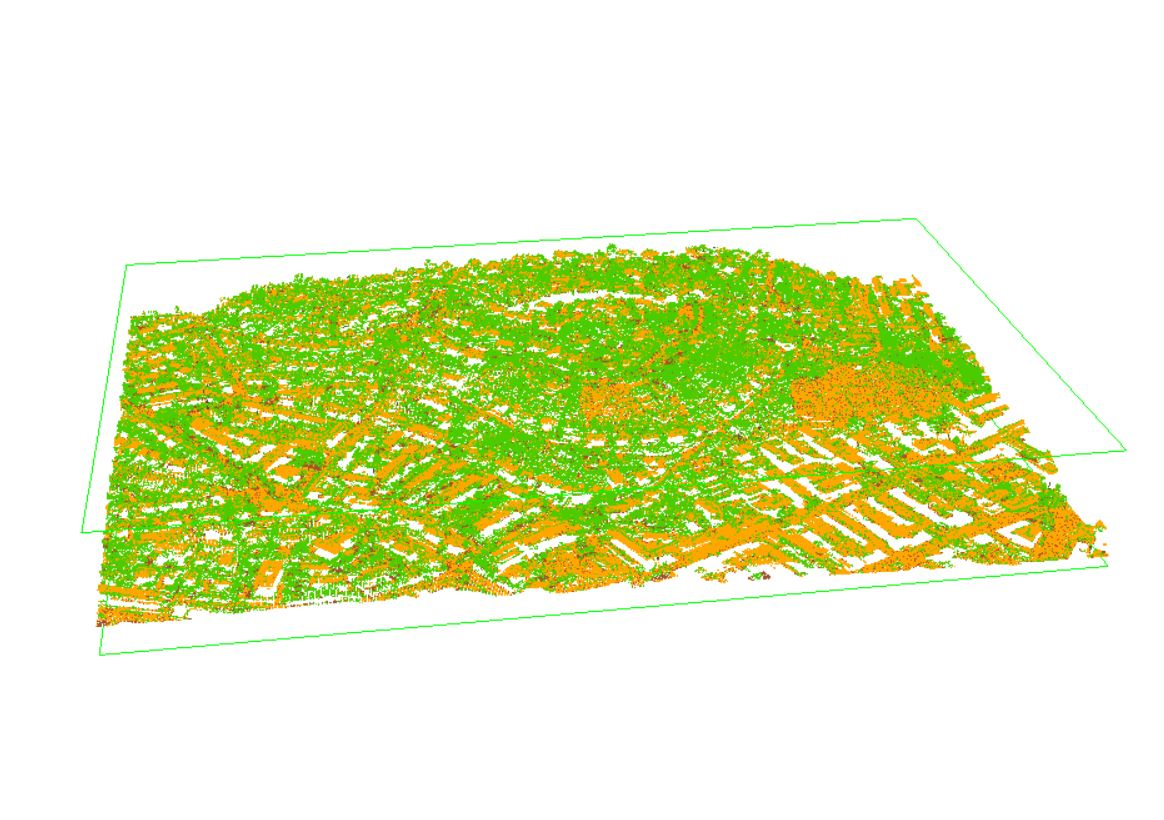
\includegraphics[width=.7\linewidth]{output.png}
		\captionof{figure}{Output via PDAL and Jupyter Notebook}
		\label{fig:output}
	\end{minipage}
\end{figure}
Figure \ref{fig:output} shows the results of the pipeline.  As we can see, the buildings are yellow and the vegetation is green.  There seems to be misclassification between some ground returns and buildings.  This can be avoided by changing some of the parameters with the filter.  Note that instead of using a progressive morphological filter I used a simple morphological filter, which is based on the progressive morphological filter. Also note that cars would not be correctly classified based on the constraints provided.
\\\\
There are different and more accurate ways to classify point clouds as noted in section \ref{sec:intro}.  Better methods include segmenting point clouds into different objects and using machine learning techniques.  Some of these methods include support vector machine and deep neural networks.  These methods are a more nuanced approach to point cloud classification.  However, shape can play a vital role in point cloud segmentation and classification.  The algorithm completed in this project is but a stepping stone to a more robust point cloud classification algorithm.    
\\\\

\section{Conclusion}
PDAL is an effective program of analyzing point clouds when looking to segment ground returns and generate approximate shapes to points.  It's highly versatile in that it's open source and can be effectively used in a data science language like Python.  As far as a simple classifier, rank estimation can have good results in very particular scenes where the user knows the environment only has a few elements such as buildings and vegetation.  As noted in section \ref{sec:results}, it is only the introductory step in a more robust and nuanced classification algorithm.
\\\\
The next step in the process is developing more robust classification techniques.  As this is an aerial collect, we can apply image segmentation algorithms to detect objects or use 3d region growing algorithms to segment point clouds.  As Rabbani, et. al. indicate, one can use the curvature (smoothness) as well as the angles between normal vectors to determine segments of point clouds \cite{rabbani2006segmentation}.  Segmentation using height, intensity, and curvature is another method.  After that, we can use a support vector machine as outlined in \cite{varney} to classify point clouds.  This, however, is beyond the scope of this project.  Future work will accomplish this either via image processing or using 3 dimensional segmentation of point clouds. 
\newpage
\bibliographystyle{plain}
\bibliography{bibfile}
	
	
\end{document}